\documentclass[12pt]{article}
\usepackage[T1]{fontenc}
\usepackage[utf8]{inputenc}
\usepackage[spanish]{babel}
\usepackage{geometry}
\usepackage{listings}
\usepackage{xcolor}
\usepackage{amsmath}
\usepackage{tabularx}
\usepackage{hyperref}
\usepackage{graphicx}

\title{\Huge{Bases de datos}}
\author{Gabriel Pérez Lago}
\date{\today}

\begin{document}
\maketitle
\vspace{2cm}
\begin{figure}[h]
    \centering
    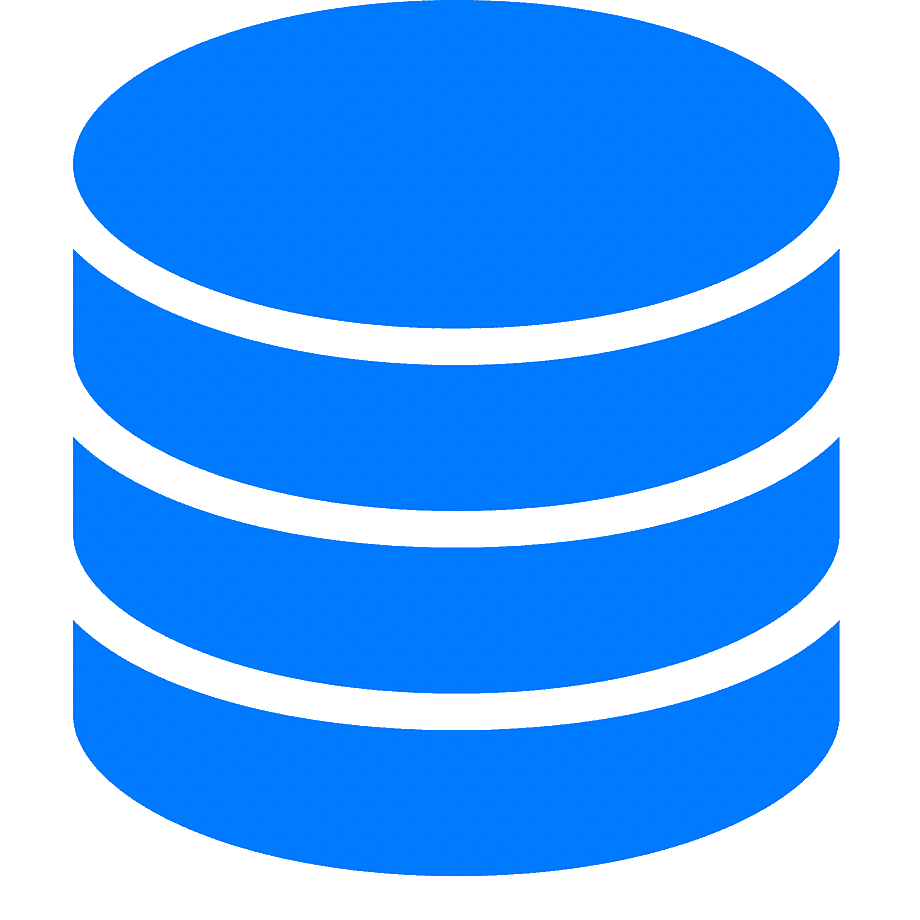
\includegraphics[width=0.5\textwidth]{./img/baseDatosd.png}
\end{figure}
\newpage
\tableofcontents
\newpage

\section{Introduccion}
Este documento tiene como objetivo explicar las diferencias y/o todo lo que engloban las principales bases de datos.
\vspace{1cm}
\begin{enumerate}
    \item SQLite
    \item MySQL
    \item PostgreSQL
    \item MongoDB
\end{enumerate}
\vspace{1cm}

El documento explicara de cada una de las bases de datos anteriormente mencionadas:

\begin{itemize}
    \item Su Historia
    \item Caracteristicas
    \item Ventajas y Desventajas
    \item Casos de Uso
    \item Un pequeño resumen final
\end{itemize}

\newpage

\begin{center}
\section{SQLite}
\end{center}

\begin{figure}[h]
    \centering
    
\includegraphics[width=0.5\textwidth]{./img/sqlite_logo.png}
\end{figure}
\vspace{1cm}
\subsection{Historia}
SQLite es unna biblioteca de base de datos de sowftware libre de tipo relacional. Esta biblioteca fue creada por \textbf{D. Richard Hipp} el \textbf{17 de agosto de 2000} para uso personal en un proyecto naval, el cual luego libero como proyecto de dominio publico y fue desarrollada principalmente en el lenguaje de programación \textit{\textbf{C}}.
SQLite buscaba ser una base de datos ligera y sencilla de implemenmtar en cualquier proyecto , sin necesidad de servidores extenros ni infrestucturas complejas , pero que tuviese la capacidad de manejar datos de manera ordenada.



\vspace{1cm}
\subsection{Caracteristicas}

SQLite es una base de datos integrada , es decir que no requiere un servidor externo para funcionar. Su sintaxis es similar a la de SQL, pero este guarda todos los datos en un solo docuemento , lo cual hace que sea mas ligera y sencilla de implementar.
Ademas es un no tiene dependencias externas, y tiene librerias de acceso para un infinidad de lenguajes de programacion y al ser de codigo fuente de dominio publico se encuentra muy bien documentada.


\vspace{1cm}
\subsection{Ventajas y Desventajas}

\textbf{Ventajas:}
\begin{itemize}
    \item Ligera y Rapida.
    \item No es requerido un servidor externo para usarla.
    \item Completamente Portatil.
    \item Se adapta a cualquier plataforma.
    \item Maneja el leguaje estandar SQL. 
\end{itemize}
\vspace{0.5cm}
\textbf{Desventajas:}
\begin{itemize}
    \item No esta pensada para alta concurrencia de datos.
    \item No es apta para aplicaciones con un alto trafico de datos.
    \item No tiene una seguridad robusta, ya que no tiene una autenticacion propia.
    \item Menor rendimiento en consultas u operaciones complejas.
\end{itemize}

\vspace{0.7cm}
\subsection{Casos de Uso}

Es una base de datos ideal para :
\begin{enumerate}
    \item Aplicaciones integradas.
    \item Aplicaciones mobiles que requieran guardar datos de manera local.
    \item Para demostraciones de aplicaciones.
    \item Almacenamiento persistentes de configuraciones y preferencias de usuarios.
    \item Para desarrollo de aplicaciones.
\end{enumerate}

\vspace{0.5cm}
\subsection{Resumen:}
SQLite es una base de datos integrada con la aplicaion , la cual la hace rapida y sencilla , pero al no tener un servidor propio esta se ve limitada al no estar capacitada para manejar altas cantidades de concurrencia de datos.

\newpage
\begin{center}
\section{MySQL}
\end{center}

\begin{figure}[h]
    \centering
    
\includegraphics[width=0.5\textwidth]{./img/mysql_logo.png}
\end{figure}
\vspace{1cm}
\subsection{Historia}
MySQL fue desarrollada por MySQL AB, una empresa sueca fundada en 1995 por \textbf{David Axmark}, \textbf{Allan Larsson} y \textbf{Michael Widenius}. MySQL AB fue adquirida por Sun Microsystems en 2008 y luego por Oracle Corporation en 2010 la cual es la empresa que mantiene la base de datos actualmente.
MySQL fue dasallorrada en el lenguje de programacion \textit{\textbf{C}} y \textit{\textbf{C++}}  y fue lanzada inicialmente en el año \textbf{2001}.
Este es un sistema de base de datos de codigo abierto y es una de las mas populares en el mundo.

\vspace{1cm}
\subsection{Caracteristicas}
MySQL es un sistema de base de datos de codigo abierto y como se dijo anteriormente es una de las mas populares en el mundo. MySQL sigue un esquema de base de datos relacional usando el lenguiaje SQL. MySQL almacena los datos mediante un sistema de tablas de filas y columnas organizadas en un esquema. Los esqumas definen la organización de la base de datos y define la relacion entra las tablas.
Dado que MySQL es de código abierto, incluye numerosas características desarrolladas en estrecha cooperación con una comunidad de usuarios durante casi 30 años. Dos capacidades en las que los desarrolladores confían son el soporte y la capacidad de escalado de MySQL. Al ser de tipo relacional la hace bastante restrictiva en cauanto al manejo y la insercion de datos. Pero esto lo soluciona con su alta consistencia y robustez.

\vspace{1cm}
\subsection{Ventajas y Desventajas}
\textbf{Ventajas:}
\begin{itemize}
    \item Es una buena opcion para alta concurrencia de datos.
    \item Tiene un buen rendimiento en consultas y operaciones complejas.
    \item Es escalable lo que implica que es una buena opcion tanto para proyectos pequeños como para proyectos grandes.
    \item Tiene una seguridad robusta.
    \item Tiene una buena documentacion.
    \item Integracion con numerosos lenguajes de programacion.
\end{itemize}
\vspace{0.5cm}

\textbf{Desventajas:}
\begin{itemize}
    \item Al contrario que SQLite MySQL requiere un servidor externo para funcionar.
    \item Algunas caracteristicas de MySQL requieren un pago.
    \item Puede limitar el manejo de datos al ser de tipo re
\end{itemize}
\vspace{1cm}
\subsection{Casos de Uso}
MySQL es una base de datos ideal para:
\begin{enumerate}
    \item Aplicaciones web tradicionales.
    \item Apis REST.
    \item ERPS y Sistemas de gestion empresarial.
    \item Aplicaciones de infraestructura compleja.
    \item Aplicaciones de alta concurrencia.
\end{enumerate}

\subsection{Resumen:}
MySQL es un sistema de base de datos ideal si quieres una base de datos robusta, escalable y con una ifraestructura bien definida. Pero en ocasiones te puede limitar en cuanrto a al libre albedrio de manejo de datos.

\newpage
\begin{center}
\section{PostgreSQL}
\end{center}

\begin{figure}[h]
    \centering
    
\includegraphics[width=0.5\textwidth]{./img/postgres_logo.png}
\end{figure}
\vspace{1cm}
\subsection{Historia}
PostgreSQL o tambien conocido como Postgrs es un sistema de base de gestión de bases de datos orientado a objetos , y como la gran mayoria es de codigo abierto.
El desarrollo de PostgreSQL no fue manejado mediante una empresa o una persona unica, sino que fue desarrollado por uan comunidad de dasarrolladores sin animo de lucro , a la cual se le denomina como \textbf{PGDG (PostgreSQL Global Development Group)}. Fue lanzada en el año \textbf{1996}. Postgres inicio su desarrolloe en el año \textbf{1986} como un proyecto universitario liderado por \textbf{Michael Stonebraker}. Y en \textbf{1996} fue lanzada la primera version estable gracias a la aportacion de persona ajenas al proyecto.

\vspace{1cm}
\subsection{Caracteristicas}
PostgreSQL es un sistema de base de datos relacional, pero este tambien soporta bases de datos no relacionales y orientado a objetos , y cumple con el estandar SQL. Postgres tiene un diseño  versatil y accesible , guardando los datos en un sistema similar al de mysql , en formatos de tablas de filas y columnas , pero este frente a mysql es muchos mas restrictivo y robusto que el anterior haciendolo mucho mas viable en cuando al manejo de gran cantidad de datos y infraestructuras complejas.

\vspace{1cm}
\subsection{Ventajas y Desventajas}
\textbf{Ventajas:}
\begin{itemize}
    \item Es una buena opcion si es necesario un manejo de altas cantidades de datos.
    \item Tiene un buen rendimiento en consultas y operaciones complejas.
    \item Soporta consultas SQL tanto avanzadas como mas sencillas.
    \item Tiene una alta concurrencia de usuarios es decir , soporta grandes cantidades de colecciones.
    \item Es una buena opcion para aplicaciones de grandes.
    \item Soporta tipos de datos avanzados : Permite usar JSON, arrays, UUID, datos geográficos, etc.
\end{itemize}
\vspace{0.5cm}

\textbf{Desventajas:}
\begin{itemize}
    \item Requiere una curva de aprendizaje mas amplia.
    \item Tiene un mayor consumo de recursos.
    \item Por su alta robustez en ocasiones puede ser un poco mas lento que MySQL.
    \item Requiere un configuración mas exigente.
\end{itemize}

\newpage
\vspace{1cm}
\subsection{Casos de Uso}
\begin{enumerate}
    \item Es muy buena opcion para CRM's.
    \item Sistemas que requieren una alta integridad.
    \item Para aplicaciones de grandes empresas o que manejan datos en muy alta concurrencia.
    \item Sistemas geospaciales.
\end{enumerate}

\vspace{1cm}
\subsection{Resumen:}
PostgreSQL es un sistema de base de datos ideal si quieres una base de datos a muy alto nivel , es perfecta para manejar muchas conexiones y trafico de datos , siendo una base de datos robusta pero en ocasiones lenta , muy recomendable para aplicaciones de alto nivel.

\newpage
\begin{center}
\section{MongoDB}
\end{center}

\begin{figure}[h]
    \centering
    
\includegraphics[width=0.5\textwidth]{./img/mongo_logo.png}
\end{figure}
\vspace{1cm}
\subsection{Historia}
MongoDB comenzó du desarrollo en el año \textbf{2007} por la empresa \textbf{10gen Inc.} ahora conocida como \textbf{MongoDB Inc.}.
Nacio de la idea de desarrollar una plataforma similar a \textbf{Google APP Engine}.
MongoDB se lanó como un producto independiente y de codigo abierto.
Pero en \textbf{Marzo} del \textbf{2011} se lanzo la version \textbf{1.4} la cual se considero la primera version estable para el uso en produccion.
\vspace{1cm}
\subsection{Caracteristicas}
MongoDB es un sistema de base de datos NoSQL y no relacional , pero tambien soporta relaciones sencillas las cuales no son tan restrictivas como puden ser las basadas en el standar SQL.
Mongo esta orientado a un manejo de datos basado en documentos , es decir que en vez de guardar los datos en tablas de filas y columnas , almacena y estructura los datos en formato \textbf{BSON} el cual es un formato de documento muy similar a \textbf{JSON}.
\vspace{1cm}
\subsection{Ventajas y Desventajas}

\newpage
\textbf{Ventajas:}
\begin{itemize}
    \item Al no ser de tipo relacional , la hace mas flexible en cuanto al almacenamiento de datos.
    \item Al ser poco restrictivo tiene un manejo de datos y una respuesta bastante rapida.
    \item Ideal para datos mutables , es decir que pueden cambiar.
    \item Estructuración sencilla al ser similar a Json.
    \item Se intengra muy bien con applicaciones modernas.
    \item No requiere una compleja Infraestriuctura.
\end{itemize}

\textbf{Desventajas:}
\begin{itemize}
    \item Al no ser relacional , en ocasiones puede ser limitante en cuanto al manejo de datos parejos entre ellos.
    \item No es recomendable para infraestructuras complejas.
    \item Permite la duplicacion de datos.
    \item No es realmente restrictivo mediante al menejo de datos.
\end{itemize}

\vspace{1cm}
\subsection{Casos de Uso}

\begin{enumerate}
    \item Buena opcion para API's sencillas.
    \item Ideal para aplicacciones en produccion.
    \item Buena opcion para Microservicios.
    \item Buena opcion para apps en tiempo real por su alta velocidad.
\end{enumerate}

\subsection{Resumen:}
MongoDB es un tipo de base de datos que se sale de los estandares , y que para aplicaciones sencillas o que requiren una trafico rapido de datos simples es excelente , pero que a la hora se ser implementada en infraestructuras complejas no es realmente aplicable.
\newpage
\section{Opinion Personal:}
Personalmente creo que este trabajo me parece super util para aprender a identificar los tipos de bases de datos que mejor se adapten a tu proyecto. Pienso que cada tipo de base de datos esta pensado para un uso especifico y que realmete todas son utiles dentro de su ambito idependientemente de su complejidad o su curva de aprendizaje.


\end{document}
